\section{Method}
\subsection{Preliminary}
Latent diffusion models~\cite{rombach2022high, ho2020denoising, peebles2023scalable} conduct a series of diffusion and denoising processes in latent space. 
%
Given a clean latent code $x_0$ from the training data, a noisy latent $x_t$ is obtained by adding an random noise $x_0\sim \mathcal{N}(0, I)$ to $x_0$ according to a timestep $t\in [0, 1]$. 
%
Following the flow matching paradigm~\cite{lipman2023flow,esser2024scaling}, $x_t$ is defined as
%
\begin{equation}  
x_t = t x_1 + (1 - t) x_0.
\end{equation}
%
The training objective of the model is to predict the velocity $v_t$, thus, the loss function of the training process can be formulated as
%
\begin{equation}  
L = \mathbb{E}_{x_0, x_1, c_{txt}, t} \left\lVert u(x_t, c_{txt}, t; \theta) - v_t \right\rVert^2,
\end{equation}
%
where $c_{txt}$ is the text condition, $\theta$ is the model weights, $u$ is the predicted velocity and $v_t$ is the ground truth velocity.

% \subsection{ERP or CP ?}
% Latent diffusion models encode the input data into latent space through VAEs.
% %
% Therefore, we first examine the reconstruction quality for the two representations, ERP and CP, to reveal which representation is better to choose within the modern diffusion paradigm.
% %
% The details of the experiments are given in Section 4. 
% %
% The experiments show that CP has better reconstruction quality compared to ERP. 
% %
% However, CP lacks an explicit representation of global spatial information. 
% %
% For example, deducing a specific 3D object from given three orthographic views is not an easy task, while the panorama spatial information in CP is implicitly contained within each face.



\begin{figure}[!h]
  \centering
    % \vspace{-1.0cm}
  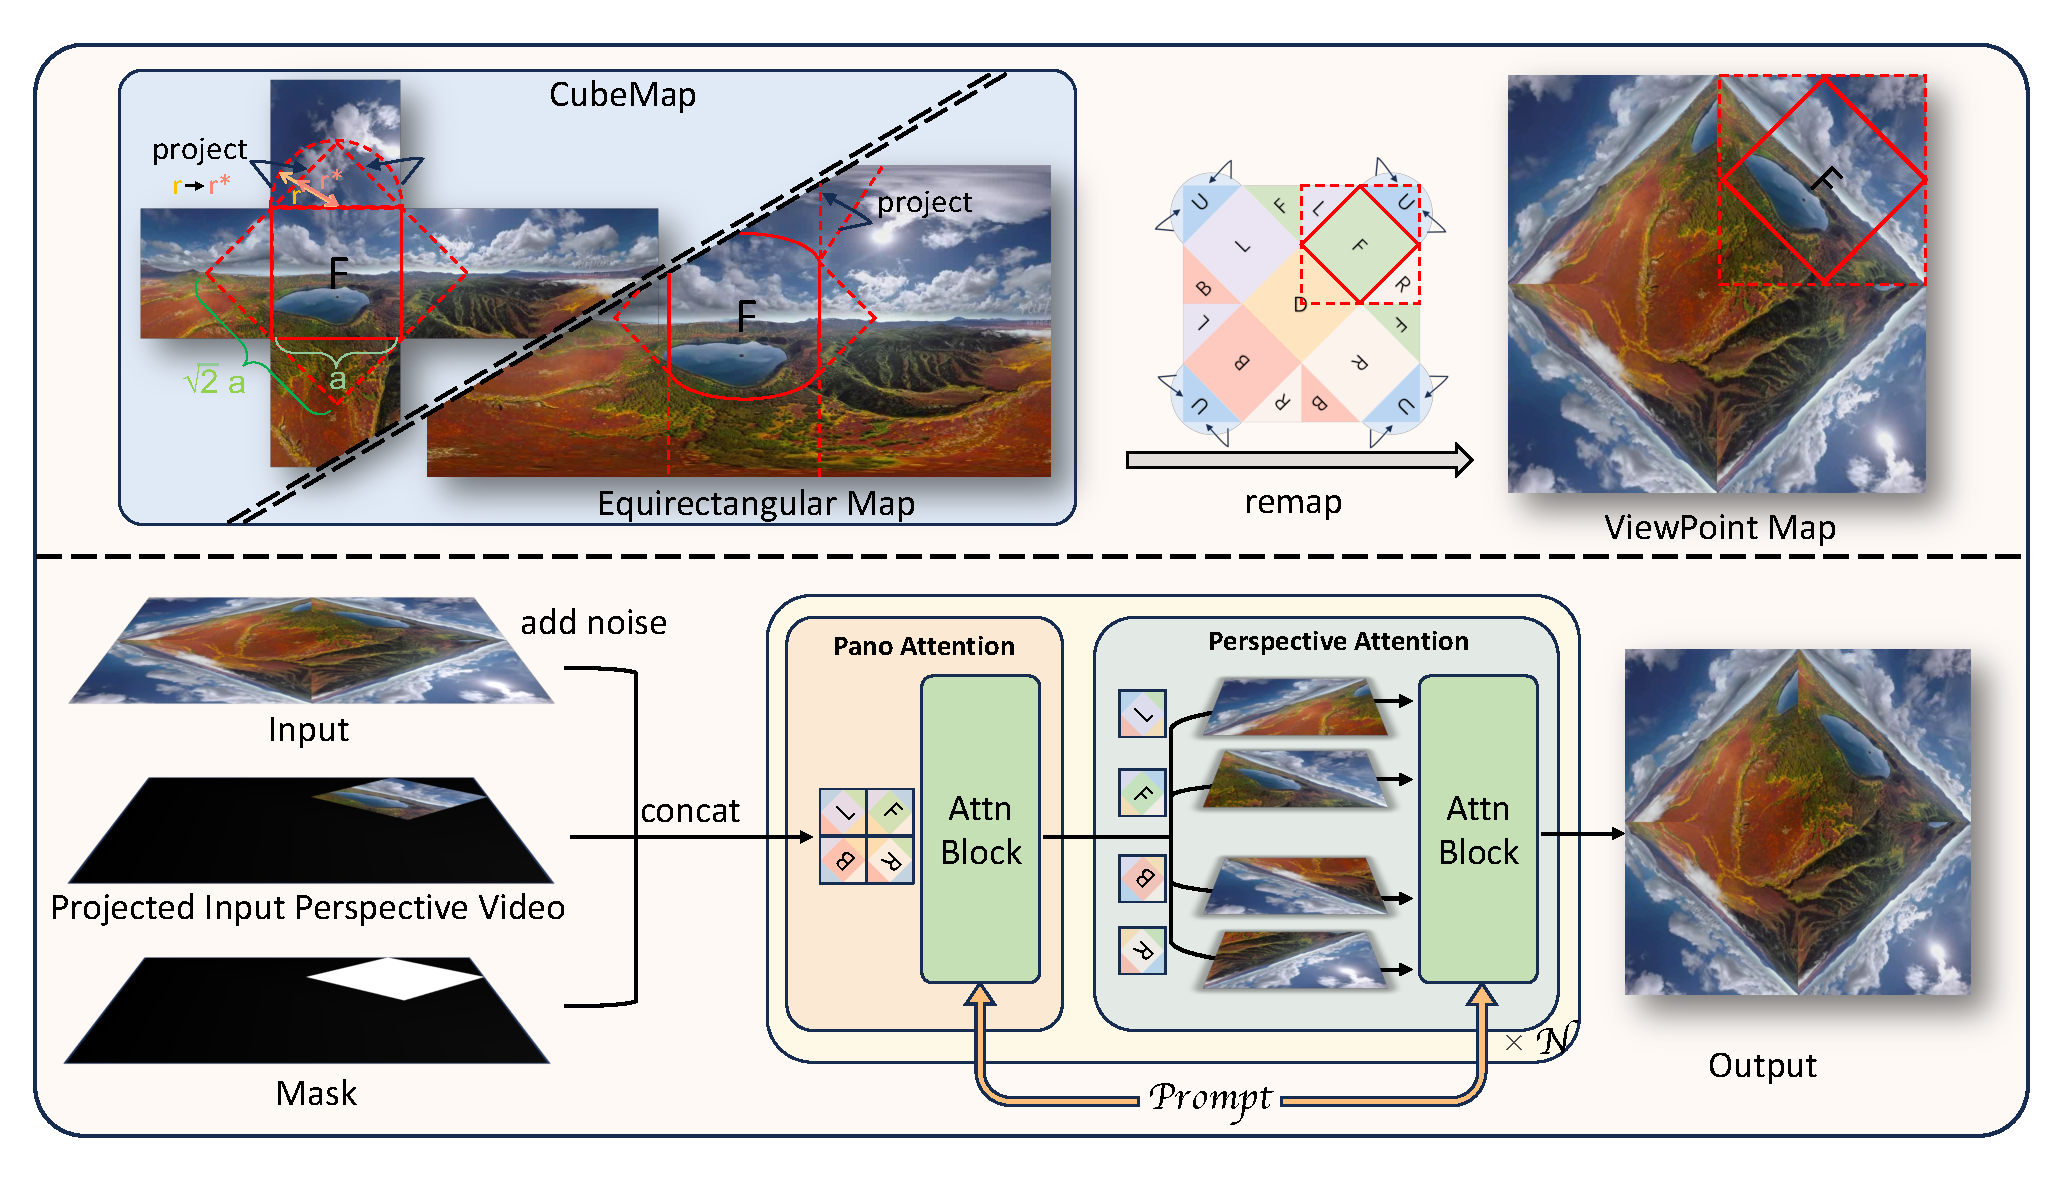
\includegraphics[width=1\linewidth]{figs/pipeline4.pdf}
    \vspace{-5.5mm}
  \caption{\textbf{Method overview.} The first row illustrates how to construct a Viewpoint map from a CubeMap or an Equirectangular Map. We begin by constructing subregions, using $\mathcal{F}$ as an example to create a pseudo-perspective region centered around it. Subsequently, we combine the four subregions to form a ViewPoint map. The second row shows the pipeline design: we first concatenate the noisy Viewpoint map, input video, and relevant mask along the channels dimension, and then employ a Pano-Perspective attention mechanism to learn how to maintain global spatial consistency while modeling fine-grained visual information.}
  \label{fig:pipe}
  % \vspace{-0.5cm}
\end{figure}

% To overcome the shortcomings mentioned above, we propose a new paradigm named ViewPoint,30
% which combines the advantages of ERP and CP. Specifically, we first project the panoramic views to31
% six cube faces with a FoV of 90◦ for each face, following the Cubemap format. This representation32
% ensures that each face is naturally suited for pre-trained diffusion schemes. Nevertheless, CP struggles33
% with spatial continuity due to the ordering of each cube face, as an unfolded cardboard box has at34
% most one face that is surrounded by four adjacent faces, thereby limiting the neural network’s ability35
% to model spatial consistency. To mitigate this limitation, we propose a pseudo-perspective view by36
% selecting one face as the central face (assuming the side length of r), then diagonally dividing each of 
% the four adjacent faces into four parts, as shown in Figure 1, and combining them into a new square 
% with the side length of √2r. This design makes the central face more spatially continuous with the 
% four adjacent faces. We then concatenate the four pseudo-perspective views centered on the left, front, 
% right, and back respectively, in raster order. The result is not only spatially consistent within each 
% pseudo-perspective region but also connects the entire cube space along the diagonals.

\subsection{ViewPoint Map}
%为了减少几何扭曲同时维持空间连续性，我们提出了...
To maintain spatial continuity while reducing spatial distortion, we propose ViewPoint Map, a novel panorama representation that combines the advantages of ERP and CP. 
%
We first sample six cube faces from either an equirectangular map or a cubemap, namely $\mathcal{F,R,B,L,U,}$ and $\mathcal{D}$, which represent the front, right, back, left, up, and down faces, respectively.
%
The four faces in the horizontal view, \ie, $\mathcal{F,R,B,L}$, typically contain most of the visual content that people focus on.
%
Therefore, we construct pseudo-perspective subregions centered around these four faces. 
%
As shown in the first row of ~\cref{fig:pipe}, we select one face as the central face (assuming the side length of $a$), then diagonally dividing each of the four adjacent faces into four parts, and finally, the central face and its four adjacent parts are concatenated to form a square region with a side length of $\sqrt[]2a$. 
%
This design makes the central face more spatially continuous with the four adjacent faces.
%
For example, if $\mathcal{F}$ is the central face, then its four adjacent faces are $\mathcal{L,R,U}$ and $\mathcal{D}$, located to the left, right, above, and below $\mathcal{L}$, respectively.
%
After obtaining the four subregions, we perform rotation and concatenation on them to further ensure that the center of the ViewPoint Map—the $\mathcal{D}$ face—is also continuous.
%
To address the splitting of $\mathcal{U}$, we project the semicircular region on the $\mathcal{U}$ face adjacent to the central face into an equilateral right triangle.
%
Formulally, for any point $P (r, \theta)$ on the semicircular region, where $r \in [0, a]$ and $\theta \in [0, \pi]$, with $a$ being the diameter of the semicircle. The scale ratio is defined as 
\begin{equation}  
d(\theta) = \frac{a}{sin\theta+\lvert cos\theta \rvert},
\end{equation}
then the scaled radial coordinate $r^*$ is computed by
\begin{equation}  
r^* = r \cdot \frac{d(\theta)}{a}.
\end{equation}
%
This design allows the $\mathcal{U}$ faces of the four subregions to have a small overlapping portion, thereby ensuring internal consistency of the entire $\mathcal{U}$ face.

\subsection{Pano-Perspective Attention}
ViewPoint Map offers global panorama information and effectively utilizes the inherent in-context generation capabilities~\cite{lhhuang2024iclora} of diffusion models. 
%
To further accelerate convergence and exploit the priors of the base model, we propose a Pano-Perspective Attention mechanism. 
%
Specifically, Pano-Attention is responsible for contextual learning to maintain spatial consistency, while Perspective-Attention focuses on generating fine-grained visual information for each subregion.
%
As shown in the second row of~\cref{fig:pipe}, we first concatenate the noisy Viewpoint Map, the projected input perspective video, and the associated mask along the channel dimension in the latent space.
%
The shape of the concatenated features is $(batch\_size, channels, frames, height, width)$. 
%
After passing through the Pano Attention block, we reshape it to $(4 \times batch\_size, channels, frames, height/2, width/2)$ and feed it into the Perspective Attention for per-regional modeling.
%
Each attention block consists of a self-attention layer, a cross-attention layer, and an FFN, the input prompt is integrated through the cross-attention mechanism.

\subsection{Overlapping Fusion}
Each subregion in a ViewPoint map has a partial spatial overlap with the two adjacent subregions. 
%
To achieve smoother transitions between subregions, we propose a gradient fusion mechanism.
%
As shown in~\cref{fig:fusion}, the overlapping parts between two subregions form a regular rhombus, therefore we construct an overlapping fusion weight $W\in \mathbb{R}^{n\times n}$ where the values decay from the area near the central face to the edges.
%
\begin{figure}[!h]
  \centering
    % \vspace{-1.0cm}
  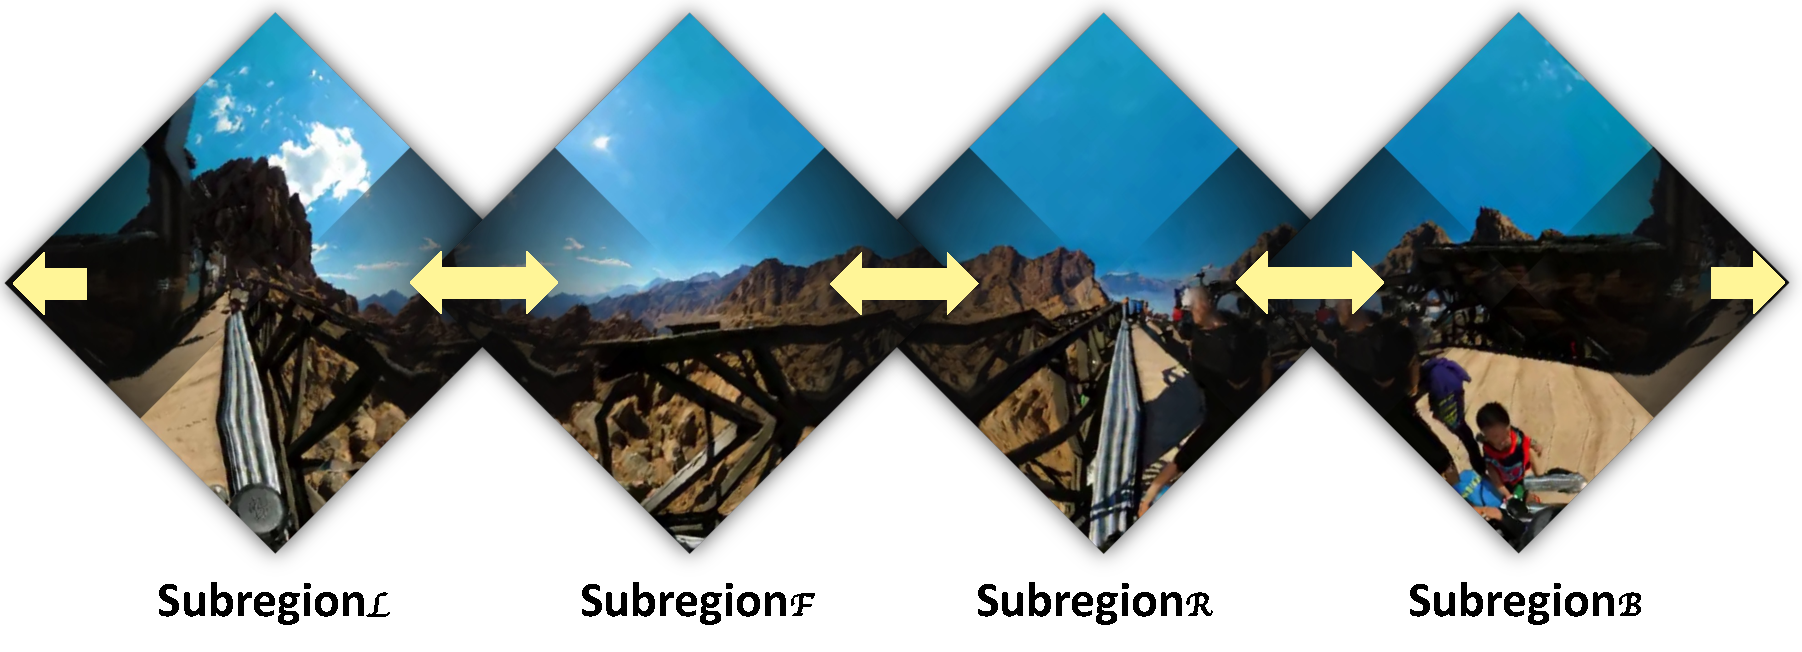
\includegraphics[width=0.8\linewidth]{figs/fusion.pdf}
  \caption{\textbf{Overlapping fusion.} The four subregions partially overlap with each other, thus we propose a gradient fusion mechanism to interpolate the overlapping areas, thereby enhancing spatial consistency.}
  \label{fig:fusion}
  %\vspace{-0.5cm}
\end{figure}

For each subregion $S_d\in \mathbb{R}^{r\times r}$, $r=2n$, $d \in [\mathcal{L,F,R,B}]$, the overlapping fusion process can be described by the following formulas:
\begin{equation}  
W_{i,j} = \frac{i+j-2}{2(n-1)}, \quad i, j = 1, 2, \dots, n
\end{equation}
where $i, j$ denote the row and column indices, respectively. Next, we define rotation. For a given matrix $A$, we have
\begin{equation}  
R_{90}(A)= A^T \cdot J, %顺时针 
\end{equation}
\begin{equation}  
R_{-90}(A)=  J \cdot A^T ,  %逆时针
\end{equation}
\begin{equation}  
R_{180}(A)=  J \cdot A \cdot J ,  %180
\end{equation}
where $J$ is the exchange matrix. Finally, for each subregion, we have
% L
\begin{equation}  
S_{L_{i,j}}=\begin{cases}
S_{L_{i,j}} \cdot R_{90}(W) + R_{-90}(S_F)_{i+n,j-n} \cdot R_{-90}(W) \text{ , } (i,j)\in [1,n]\times [n+1,r] \\
S_{L_{i,j}} \cdot R_{-90}(W) + R_{90}(S_B)_{i-n,j+n} \cdot Rot_{90}(W) \text{ , } (i,j)\in [n+1,r]\times [1,n]\\
\end{cases}
\end{equation}
% R 
\begin{equation}  
S_{R_{i,j}}=\begin{cases}
S_{R_{i,j}} \cdot R_{90}(W) + R_{90}(S_F)_{i+n,j-n} \cdot R_{-90}(W) \text{ , } (i,j)\in [1,n]\times [n+1,r] \\
S_{R_{i,j}} \cdot R_{-90}(W) + R_{-90}(S_B)_{i-n,j+n} \cdot R_{90}(W) \text{ , } (i,j)\in [n+1,r]\times [1,n]\\
\end{cases}
\end{equation}
% F 
\begin{equation}  
S_{F_{i,j}}=\begin{cases}
S_{F_{i,j}} \cdot W + R_{90}(S_L)_{i+n,j+n} \cdot R_{180}(W) \text{ , } (i,j)\in [1,n]\times [1,n] \\
S_{F_{i,j}} \cdot R_{180}(W) + R_{-90}(S_R)_{i-n,j-n} \cdot W \text{ , } (i,j)\in [n+1,r]\times [n+1,r]\\
\end{cases}
\end{equation}
% B
\begin{equation}  
S_{B_{i,j}}=\begin{cases}
S_{B_{i,j}} \cdot W + R_{-90}(S_L)_{i+n,j+n} \cdot R_{180}(W) \text{ , } (i,j)\in [1,n]\times [1,n] \\
S_{B_{i,j}} \cdot R_{180}(W) + R_{90}(S_R)_{i-n,j-n} \cdot W \text{ , } (i,j)\in [n+1,r]\times [n+1,r]\\
\end{cases}
\end{equation}
%
Note that we apply overlapping fusion to each subregion simultaneously, rather than in the order specified in the above formulas.

For the $\mathcal{U}$ face, we first project the triangles back into semicircles and transform the rhombus into a petal shape formed by the overlap of two circles. 
%
Finally, we use a similar fusion mechanism to fuse the overlapping of the four semicircles.
